%!TEX root = ../main.tex

\subsection{FePO$_4$}
\label{ssec:phosphate}

The third absorber that is placed in the $\gamma$-source beam path is the iron
compound FePO$_4$. The Mössbauer spectrum of FePO$_4$ displays two characteristic
absorption peaks that are closely located. This is shown in \autoref{fig:phosphate}.
The fit parameters of the optimisatisation are given in \autoref{tab:phosphate}.

The isometric shift of FEPO$_4$ is given by \autoref{eq:iso-shift-phosphate} and has
again been calculated in the same process as lined out in \autoref{ssec:iron}.

\begin{equation}
\label{eq:iso-shift-phosphate}
\Delta E = -\SI{103.040\pm6.571e-10}{\electronvolt}.
\end{equation}

In an attempt to quantify the electric field gradient $\frac{\partial E}{\partial z}$
= $\frac{\partial^2 V}{\partial z^2}$ along the axis of the permeating magnetic
field, the number of and distance between absorption peaks is analysed in more
detail. These observables are influenced by the \textbf{quadrupole} shift. Following
the derivation in \cite{Sch17}, the energy by which a state with nuclear spin $I$ and
magnetic moment $m$, and electric quadrupole moment $Q$ is altered calculates as

\begin{equation}
\label{eq:quadrupole-shift}
\Delta E_Q(I,m) = \frac{e\cdot Q}{4}\;\frac{3m^2-I\cdot(I-1)}{3I^2-I\cdot(I+1)}\,\frac{\partial^2V}{\partial z^2}.
\end{equation}

Owed to the material properties of FePO$_4$ and FeSO$_4$ in the following subsection,
and taking into account the Doppler shift of the high-energy $\gamma$'s,
\autoref{eq:quadrupole-shift} can be rewritten so that the electric field gradient
can be obtained from the location $v$ of absorption peaks.

\begin{equation*}
	\Delta E_Q(\frac{3}{2},\pm\frac{3}{2}) = +\frac{e\cdot Q}{4}\;\frac{\partial^2 V}{\partial z^2},\qquad \Delta E_Q(\frac{3}{2},\pm\frac{1}{2}) = -\frac{e\cdot Q}{4}\;\frac{\partial^2 V}{\partial z^2}
\end{equation*}

\begin{align*}
\Delta v &= v(\frac{3}{2},\pm\frac{3}{2}) - v(\frac{3}{2},\pm\frac{1}{2}) = \frac{e\cdot Q}{2}\cdot\frac{c}{E_0}\cdot\frac{\partial^2 V}{\partial^2 z} \\
\Leftrightarrow\qquad\frac{\partial^2 V}{\partial^2 z} &= \frac{2E_0}{e\cdot Q\cdot c}\;\;\Delta v.
\end{align*}

With the given quadrupole moment $Q=\SI{0.21\pm0.01e-28}{\meter\squared}$ from 
\cite{Sch17}and the location of the absorption peaks as listed in 
\autoref{tab:phosphate}, the electric field gradient is found to be

\begin{equation}
\label{eq:field-gradient}
\frac{\partial^2 V}{\partial^2 z} = \SI{2.3673\pm0.149e24}{\volt\per\meter\squared}.
\end{equation}

This corresponds to an electric field strength of roughly 
$\SI{2.36e14}{\volt\per\meter}$ across characteristic length scales of an atom (
\SI{e-10}{\meter}).

\begin{figure}
	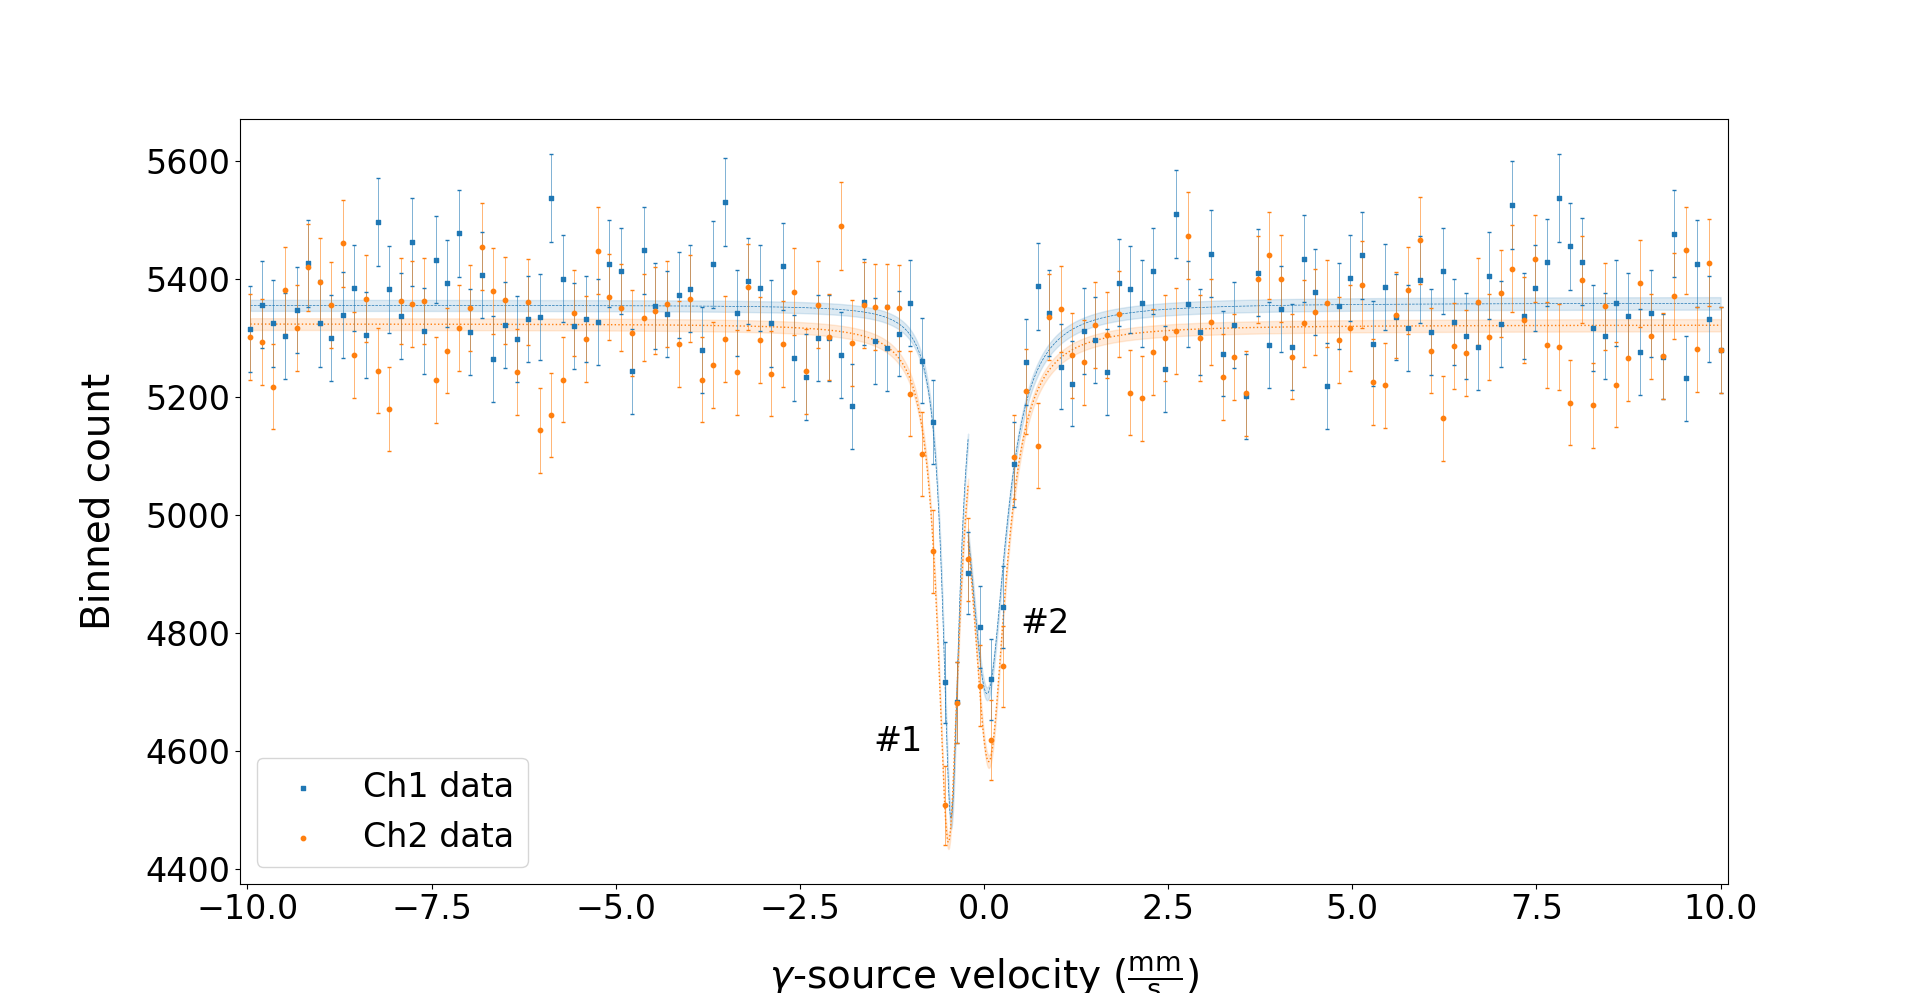
\includegraphics[width=1.0\textwidth]{./fig/Phosphate.png}
	\caption{Mössbauer spectrum of FePO$_4$}{}
	\label{fig:phosphate}
\end{figure}

\begingroup
\renewcommand{\arraystretch}{1.3}
\begin{table}
	\begin{center}
	\caption{Mössbauer spectrum fit parameters for phosphate}
	\begin{tabular*}{0.9\textwidth}{@{\extracolsep{\fill}} c|ccccc}
  \toprule
	\hline
  Peak \# & $\Upphi_0$ & $A$ & $v_0$ & $\Gamma$ & Channel \\
	\hline
  \multirow{2}{*}{\#1} & $5355\pm9$ & $16\pm7.1$ & $-0.45\pm0.01$ & $0.275\pm0.080$ & Ch1 \\
                       & $5323\pm10$ & $28\pm7.4$ & $-0.48\pm0.02$ & $0.358\pm0.057$ & Ch2 \\
                       \hline
  \multirow{2}{*}{\#2} & $5359\pm11$ & $64\pm17.9$ & $0.04\pm0.03$ & $0.622\pm0.103$ & Ch1 \\
                       & $5322\pm10$ & $57\pm13.9$ & $0.06\pm0.02$ & $0.557\pm0.080$ & Ch2 \\
                       \hline
    \bottomrule
		\end{tabular*}
		\label{tab:phosphate}
	\end{center}

\end{table}
\endgroup

